%% LyX 2.3.5.2 created this file.  For more info, see http://www.lyx.org/.
%% Do not edit unless you really know what you are doing.
\documentclass[12pt,english]{article}
\usepackage{fourier}
\usepackage[T1]{fontenc}
\usepackage[latin9]{inputenc}
\usepackage[letterpaper]{geometry}
\geometry{verbose,tmargin=2cm,bmargin=2cm,lmargin=2cm,rmargin=2cm}
\usepackage{color}
\usepackage{babel}
\usepackage{textcomp}
\usepackage{amsmath}
\usepackage{graphicx}
\usepackage{rotfloat}
\usepackage{setspace}
\usepackage[authoryear,round]{natbib}
\usepackage{subscript}
\usepackage{microtype}
\onehalfspacing
\usepackage[unicode=true,
 bookmarks=true,bookmarksnumbered=false,bookmarksopen=false,
 breaklinks=true,pdfborder={0 0 0},pdfborderstyle={},backref=false,colorlinks=true]
 {hyperref}
\hypersetup{
 pdfauthor={Andrea Manera, Michele Fornino},
 allcolors = blue}

\makeatletter

%%%%%%%%%%%%%%%%%%%%%%%%%%%%%% LyX specific LaTeX commands.
%% Because html converters don't know tabularnewline
\providecommand{\tabularnewline}{\\}
%% A simple dot to overcome graphicx limitations
\newcommand{\lyxdot}{.}


%%%%%%%%%%%%%%%%%%%%%%%%%%%%%% User specified LaTeX commands.
\usepackage[bottom]{footmisc}
\usepackage{pifont}
\usepackage{placeins}
\usepackage{tabularx}
\usepackage{booktabs}

\newcolumntype{C}[1]{>{\centering\let\newline\\\arraybackslash\hspace{0pt}}m{#1}}
\newcolumntype{L}[1]{>{\flushleft\let\newline\\\arraybackslash\hspace{0pt}}m{#1}}
\newcolumntype{P}{>{\centering\arraybackslash}m{3cm}}
\renewcommand{\baselinestretch}{1.3} 

\@ifundefined{showcaptionsetup}{}{%
 \PassOptionsToPackage{caption=false}{subfig}}
\usepackage{subfig}
\makeatother

\begin{document}

\section{Data description\label{sec:Data-description}}

In this section, I detail source material and the construction of
the dataset used in my empirical analysis. Subsection \ref{subsec:Data-Sources}
lists the sources of the raw data. Subsection \ref{subsec:KnowledgeMarkets}
focuses on the definition of inventor productivity measures and knowledge
markets, which I identify through realized inventor flows across sectors.
Subsection \ref{subsec:Other data and aggregation} briefly describes
other data construction steps that are discussed in more detail in
Appendix \ref{app: Data-Construction-Details}.

\subsection{Data Sources\label{subsec:Data-Sources}}

My empirical analysis relies on the variation of concentration across
product markets, as defined by 4-digit NAICS sectors, the impact of
these shifts on the allocation of inventors with specific competences
across these sectors, and the subsequent effect on inventor productivity.
I use USPTO patent data to measure inventor productivity and establish
the set of product markets that share similar inventors, and US Economic
Census data to obtain concentration and productivity growth measures.
Finally, I also use a dataset of product market regulations, Mercatus
RegData 4.0, to conduct an instrumental variable analysis, as well
as NBER-CES to obtain estimates of the Lerner Index that I employ
in the calibration of my theoretical model.

My primary source is USPTO patent data from PatentsView. This dataset
contains disambiguated patent, inventor, and assignee identifiers,
as well as Cooperative Patent Classification (CPC) classes for each
of the patents registered from1975 to 2021. I then identify inventor
flows across different sectors, employing the ALP classification of
1976-2016 patents into NAICS sectors of application developed by \citet{goldschlagAlgorithmicLinksProbabilities2016}.
Since this classification is constructed using the PATSTAT dataset,
I rely on the crosswalk built by Gianluca Tarasconi to match these
two sources.\footnote{See \href{https://patentsview.org/forum/7/topic/143}{https://patentsview.org/forum/7/topic/143},
\href{https://rawpatentdata.blogspot.com/2019/07/patstat-patentsview-concordance-update.html}{https://rawpatentdata.blogspot.com/2019/07/patstat-patentsview-concordance-update.html}} This leaves me with one third of all the patents registered between
1975 and 2021, due to the restriction of the time frame to 1976-2016
and an incomplete match between PATSTAT and PatentsView. I comb patent
records for self-citations, truncation-corrected forward citations,
and patent generality, following the procedure in \citet{hallNBERPatentCitation2001}
and \citet{acemogluRadicalIncrementalInnovationForthcoming}. I restrict
my attention to utility patents, as I am interested in patents with
a technological content and not just design improvements.

My main source for concentration and sales data is the US Economic
Census (EC), which reports sales shares for the top 4, 8, 20, and
50 firms; the Herfindal-Hirschman Index; sales and number of companies
in various NAICS 4-digit sectors at a 5-year frequency. I restrict
my attention to the period between 1997 and 2012 for three main reasons.
First, as I show below, this period saw substantial increase in the
concentration of inventors in specific technology classes. Second,
the start of this period coincides with an acceleration in the growth
of market concentration and markups \citep[see,  e.g., ][]{deloeckerRiseMarketPower2020}.
Third, 1997 saw the adoption of the NAICS classification, thus ensuring
a consistent definition of product markets throughout the period I
analyze As my baseline concentration measure, I rely on the HHI lower
bound constructed by \citet{keilTroubleApproximatingIndustry2017}.\footnote{Available at \href{https://sites.google.com/site/drjankeil/data.}{https://sites.google.com/site/drjankeil/data.}}
I did so because the Economic Census reports the HHI only for a subset
of industries, which would severely limit my sample. The method proposed
by \citet{keilTroubleApproximatingIndustry2017} obviates this issue
by constructing the implied lower bound of the HHI implied by top
sales shares reported in the Economic Census, which are available
for a much wider set of industries than the HHI.\footnote{As detailed in \citet{keilTroubleApproximatingIndustry2017} this
measure is very strongly correlated with the HHI reported by the Economic
Census when this is available, with a correlation of around 0.93.} While my estimates are robust to using the EC-reported HHI, this
choice allows me to obtain more power for my findings as well as to
generalize them.

The Economic Census also provides sector-level growth in output per
worker, which constitutes my main measure of productivity growth.
I choose this measure instead of multi-factor productivity since the
latter is available only for a limited set of sectors, mostly in manufacturing.
I deflate sales using NAICS-specific price indices from the Bureau
of Labor Statistics.

I employ two additional data sources in the empirical analysis and
in the calibration of my model. First, I obtain sector-specific counts
of regulations for various NAICS 4-digit sector from the Mercatus
RegData 4.0 dataset. I employ them to conduct an instrumental variable
analysis, strengthening the causal interpretation of my results.\footnote{Available at https://www.quantgov.org/bulk-download.}
Second, I use NBER-CES data to produce estimates of the Lerner Index
following \citet{grullonAreUSIndustries2019a}.

All told, out of a total of 304 NAICS 4-digit sectors, I have assembled
157 business sectors for which I can measure the interrelation between
concentration and knowledge markets.

\subsection{Effective Inventors and Knowledge Markets\label{subsec:KnowledgeMarkets}}

The main aim of this section is grouping product markets that share
the same \emph{required} \emph{knowledge to innovate} and therefore
compete for the same R\&D inputs, namely inventors. I identify sectors
that routinely exchange researchers through the Louvain community-detection
algorithm \citep{blondelFastUnfoldingCommunities2008}.

Figure \ref{fig: KmarketGraph} illustrates how I construct knowledge
markets. Each node in the Figure represents a different NAICS 4-digit
sector, and the black lines designate the inventor flows. The procedure
shows how I determine these flows and measure their strength. After
obtaining these weighted flows, I employ a community detection algorithm
to group together sectors most closely connected. Figure \ref{fig: KmarketGraph}
depicts strong flows among grain, vegetable farming and animal food
manufacturing, all of which involve knowledge related to agriculture
and nutrition, and separately between footwear and tanning, which
both require knowledge of leather crafting. In this case, my algorithm
would identify two knowledge markets, one given by the agriculture
and food manufacturing sectors, and the other by leather crafting
sectors, leaving the laundry services sector isolated. Based on the
strength of connections, we would expect increased concentration in
footwear manufacturing to attract inventors away from leather tanning,
but not from vegetable farming. Increased concentration in the laundry
sector, which has weak ties to the other sectors, would lead to negligible
inventor movement within this particular grouping.

\begin{figure}[t]
\caption{Graphical Illustration of Knowledge Markets}
\label{fig: KmarketGraph}
\begin{centering}
\includegraphics[width=0.9\textwidth]{../graphs/Kmarkets/Kmarkets\lyxdot 006}\\
\par\end{centering}
{\footnotesize{}Note: This figure provides a graphical illustration
of the definition of knowledge markets as sets of product markets
sharing the same required knowledge to innovate. This illustration
is based on transitions of inventors across product markets observed
in my data and classified in the same knowledge markets, although
many other sectors in these markets are excluded for the sake of exposition.
In the figure, nodes represent NAICS sectors 1111 (Oilseed and Grain
Farming), 1112 (Vegetable and Melon Farming), 3111 (Animal Food Manufacturing),
3161 (Leather and Hide Tanning and Finishing), 3162 (Footwear Manufacturing),
and 8123 (Drycleaning and Laundry Services). The edges connecting
nodes represent inventor transitions across sectors, while the width
of these edges represents the strength of the connection between the
two sectors as measured by undirected inventor flows.}{\footnotesize\par}
\end{figure}


\paragraph{Measuring Inventor Transitions}

I employ the USPTO patent data classified into 4-digit NAICS sectors
by \citet{goldschlagAlgorithmicLinksProbabilities2016} to construct
knowledge markets. Table \ref{tab:Data} depicts a hypothetical matching
of the USPTO dataset with NAICS classifications. Note that the first
patent has multiple inventors and is applicable to multiple sectors.
Inventors are each assigned a disambiguated ID corresponding to the
serial number of their first patent. In this example, inventor 00001-1
and 00001-2 both cooperate on the development of patent US00001. The
third column in Table \ref{tab:Data} shows the \citet{goldschlagAlgorithmicLinksProbabilities2016}
classification for NAICS 4-digit industries. This classification is
not limited to a single sector per patent, and includes multiple sectors
in almost all instances. For instance, patent US00001 relates to multiple
sectors, while patent US00002 is applicable to just one sector. Importantly,
this classification captures the \emph{technological nature} of the
patent and the sectors of application of the knowledge required to
develop that patent. While other classifications, like the CPC or
the USPC, also describe the technological nature of patents, they
do not allow a direct match to sectors of application.

Given this data structure, I define a transition in two ways. First,
I consider inventor transitions \emph{within patents.} That is, I
consider that an inventor transition occurs between two sectors if
an inventor works on a patent that applies to both. The direction
of flows does not matter for the definition of knowledge markets,
since I am only interested in grouping sectors that exchange researchers.
Table \ref{tab:Data} depicts two transitions between sectors 1111
and 1112 in 1980. The second type of transition that I consider is
\emph{across patents}. This transition occurs when an inventor applies
his knowledge to patents in different product markets, such as between
sector 1112 and 3111 by inventor 00001-1. The raw count of transitions
of inventors across sectors in each year constitutes the basis of
my measure of inventor flows.
\begin{center}
\begin{table}

\begin{centering}
\caption{USPTO Data Structure}
\label{tab:Data}%
\begin{tabular}{|c|c|c|c|}
\hline 
Patent ID & Inventor ID & \citet{goldschlagAlgorithmicLinksProbabilities2016} NAICS & Year\tabularnewline
\hline 
US00001 & 00001-1 & 1111 & 1980\tabularnewline
US00001 & 00001-1 & 1112 & 1980\tabularnewline
US00001 & 00001-2 & 1111 & 1980\tabularnewline
US00001 & 00001-2 & 1112 & 1980\tabularnewline
US00002 & 00001-1 & 3111 & 1981\tabularnewline
\hline 
\end{tabular}\\
\par\end{centering}
{\footnotesize{}Note: This table displays a hypothetical example of
the data structure employed to build knowledge markets. The columns
``Patent ID'' and ``Inventor ID'' represent disambiguated patent
and inventor identifiers as classified by USPTO PatentsView Data.
The column ``\citet{goldschlagAlgorithmicLinksProbabilities2016}
NAICS'' classifies patents into NAICS 4-digit sectors.}{\footnotesize\par}
\end{table}
\par\end{center}

\paragraph{Weighting Inventor Flows: Effective Inventors}

After identifying transitions, I proceed to weigh them by two alternative
measures in order to assess the flow of inventors across sectors.
The first measure weighs each transition equally, computing inventor
flows as the raw count of researchers moving across NAICS. The second
measure adjusts for the productivity of individual inventors, since
raw counts might overstate or understate the importance of each transition,
depending on the size of origin and destination sectors, their technological
nature, as well as the proficiency of each inventor. I therefore define
a measure of ``effective inventors'' that aims to correct for these
and other omitted factors. For each inventor,

I estimate the fixed effect, $\alpha_{i},$ in the fully-saturated
regression 
\begin{align}
\text{\#Patents}_{cfit} & =\alpha_{i}+\gamma_{cft}+\varepsilon_{cfit},\label{eq:one-1-1}
\end{align}
where $\text{\#Patents}_{cfit}$ denotes the number of patents registered
in CPC class $c$; firm (assignee) $f$; and year $t$, that include
inventor $i.$ In this regression $\gamma_{cft}$ denotes a of CPC
class by firm (assignee) by year fixed effect. I choose to include
indicators for one-digit CPC classes, the broadest classification,
to identify as many fixed effects as possible. The fixed effect $\gamma_{cft}$
controls for specific technological features of the patented technology,
the firm environment, as well as the year. Further, this specification
produces an estimate of inventor productivity that accounts for the
number of collaborators on each patent. Given this specification,
I define an \emph{effective inventor} as one unit of the resulting
fixed effect $\alpha_{i}$, rescaled to take nonnegative values. Since
these fixed effects might be inconsistently estimated, I check the
robustness of all my results, including the construction of knowledge
markets, to the use of the raw count of inventors.

Armed with the results of this estimate, I define \emph{effective
inventor flows} between sector $j$ and sector $k$ at time $t$ as:
\begin{align*}
flow_{j\rightarrow k,t} & =\sum_{i}\#\left\{ \text{\ensuremath{i\text{'s}\ \text{transitions}\ j\rightarrow k\text{ \ensuremath{\text{in}} }t}}\right\} \cdot\alpha_{i},
\end{align*}
that is, the sum of transition counts weighted by effective inventors.
The total undirected flow between two sectors is then given by the
sum of inflows and outflows with ends in one of the two sectors: 
\[
flow_{jk}=\sum_{t}\left(flow_{j\rightarrow k,t}+flow_{k\rightarrow j,t}\right).
\]
This flow measure defines a network of inventor transitions across
product markets, where the nodes, $j,k$, are given by 4-digit NAICS
codes, edges are given by transitions across sectors, and edge weights
are defined as a rescaled version of $flow_{jk}.$ I use these edge
weights as a measure of the strength of the connection between pairs
of sectors in the network. Rescaling the flow measure is necessary
in order to exclude effects of sector size as well as to avoid double
counting of inventors. I describe how I rescale this series in Appendix
\ref{app: Data-Construction-Details}.

\paragraph{Community Detection and Resulting Knowledge Markets}

I use the rescaled undirected flow measure as a network edge weight
to identify communities through the Louvain algorithm developed by
\citet{blondelFastUnfoldingCommunities2008}. This procedure maximizes
the modularity of the network by choosing the number of communities
(knowledge markets) and the assignment of nodes (NAICS sectors) to
communities. Modularity, a commonly used measure of connectedness
of networks, measures the distance between the density of links \emph{within}
communities versus \emph{between.}

This procedures produces 10 sets of NAICS 4-digit sectors that share
the same inventors and have concentration measures. Applying the community
detection algorithm results in knowledge markets that do not overlap:
Each NAICS 4-digit sector belongs to one and only one knowledge market.
Figure \ref{fig: KmarketGraph-1} displays the result of my procedure
applied to NAICS 3-digit sectors. I report this exercise since the
4-digit equivalent would be too dense to depict. However, the knowledge
markets identified by the two exercises are qualitatively similar
although they are clearly more numerous in the 4-digit case. In this
figure, lines denote inventor transitions, with width proportional
to the effective undirected inventor flow between sectors. Nodes represent
NAICS 3-digit. Black lines depict flows within knowledge markets,
while gray lines represent transitions between communities.

Three features are worth emphasizing. First, the network is very dense,
and transitions across 3-digit as well as 2-digit sectors are pervasive,
differing largely in intensity. This approach is far more illuminating
than grouping sectors based on broad product markets, which would
neglect the linkages across disparate markets, or pooling all sectors
together, which would neglect the difference in the strength of inventor
flows. Second, the flows between communities appear more numerous
than within communities, but this is solely a by-product of the circular
layout of the network, whereby nodes mask flows within close communities
on the circle. When applying the algorithm to 4-digit sectors, I find
that less than a third of flows occur between communities, as expected
since the community detection algorithm maximizes the density of within-community
linkages. Third, and perhaps most importantly, the classification
that I obtain sensibly groups together sectors that we might expect
to share similar knowledge to innovate. Starting from sector 111 and
going counter-clockwise, the knowledge markets in the figure can be
described as follows. The first market, including sector 111, groups
sectors involving agricultural production (111, 112 and 114) and food
manufacturing (311). The second market, starting with 211, includes
oil, gas, and mining. The green cluster at the top of the figure groups
several heavy manufacturing industries, such as chemicals plastics
and petroleum products, and pipeline transportation (486). The market
in yellow consists largely of transportation services and manufacturing
as well as motor vehicle dealers. The large blue cluster captures
many retail sectors, as well as data processing, telecom, and broadcasting
services. The remaining three markets include insurance and finance
(red cluster), computer, electronics, and machinery manufacturing
and professional services (violet), and wholesalers (gray).

Knowledge markets are identified using my measure of effective inventors,
but the algorithm produces nearly identical results when using raw
inventor counts; more than 97\% of 4-digit NAICS sectors are classified
in the same manner using the two measures. That is, 97\% of sector
pairs belong to the same knowledge market according to both measures.

\begin{figure}[th]
\caption{Knowledge Markets Obtained from NAICS 3-digit Sectors}
\label{fig: KmarketGraph-1}
\begin{centering}
\includegraphics[width=0.8\textwidth]{../graphs/NewCommunity_3d}\\
\par\end{centering}
{\footnotesize{}Note: This figure displays the network of inventor
flows between NAICS 3-digit sectors and the knowledge markets resulting
from the application of the Louvain community detection algorithm.
Lines denote inventor transitions, with width proportional to the
effective undirected inventor flow between sectors. Nodes represent
NAICS 3-digit sectors. Black lines depict flows within knowledge markets,
while gray lines transitions between communities.}{\footnotesize\par}
\end{figure}

\FloatBarrier

\subsection{Other Constructed Measures and Aggregation at Census Frequency\label{subsec:Other data and aggregation}}

\paragraph{Patent Citation Measures}

For each patent classified by \citet{goldschlagAlgorithmicLinksProbabilities2016},
I compute self-citations, forward citations, and a measure of patent
generality. To count self-citations, I first identify the set of cited
patents that belong to the same assignee as the citing patent. I weigh
self-citations to account for cited patents that have multiple assignees.
I count as one self-citation instances where the patent has a single
assignee, and as one half if the cited patent has multiple assignees.
The share of self-citations is given by the sum of weighted self-citations
divided by the number of patents cited by each assignee. I construct
five measures to correct self-citations for the assignee's importance
in the relevant technology class of cited patents. For each citation
made, excess self-citations are defined as $1-Pr\left(\text{self-citation}\right)$.
The measure depends on how the probability of self-citation is computed.
For the first three measures, I compute this probability as the assignee's
share of total patents in the NAICS code attributed to the citing
patent. I employ in turn the share of NAICS patents for the year of
citation, the previous five years, and the cumulative share from the
beginning of the sample. The other two measures are based on the CPC
classification at the group and subgroup levels (the lowest levels
of detail in the classification). For this measure, the probability
of self-citation is derived for each citation by taking the share
of patents by the assignee in the CPC (sub)group and the year corresponding
to the cited patents.\footnote{This procedure is similar to the approach followed in Akcigit and
Kerr's (2018) Appendix C.} Finally, I aggregate all measures across assignees in the same NAICS
4-digit code using the number of patents in the relevant code by each
assignee in each year.

I also construct two truncation-corrected forward citation measures
and a patent generality measure following the definitions and the
procedures described in \citet{hallNBERPatentCitation2001}. The forward
citation measures compute the average number of citations received
by each firm's patents, giving an indication of the importance of
each patent for future technological developments. The correction
for truncation is conducted by estimating the empirical CDF of the
forward citations lag distribution of patents in the relevant CPC
2-digit technology class. The correction is then carried out by dividing
the overall number of forward citations at the latest available date
by the inverse of the CDF thus obtained. The procedure suggested by
\citet{hallNBERPatentCitation2001} uses only information pertaining
to the CPC 2-digit technology class of the cited patent. I also conduct
an alternative correction that estimates a separate distribution for
each citing CPC 2-digit class and sums the corrected forward citations
across all citing classes. Patent generality also measures the technological
impact of patents, but rather than focusing on citations it examines
the scope of application of the patent. In particular, it measures
the dispersion of citations received across different CPC classes.
The higher the dispersion, the wider the technological applicability
of the patent.\footnote{The interested reader should consult \citet{acemogluRadicalIncrementalInnovationForthcoming}
for a detailed discussion, and the related appendix for details on
the construction of these measures.}

\paragraph{Regulation Data}

Mercatus RegData provides a count of restrictions imposed on a number
of NAICS 4-digit product markets, obtained by matching a set of keywords
in NAICS descriptions to regulatory texts, and then taking the best
match for each document. However, the available data does not include
a set of codes due to data quality reasons.

Therefore, I process the description of NAICS 4-digit codes and compute
the cosine-similarity between all pairs of sectors. I build an estimate
of sector-relevant restrictions for missing sectors by taking an average
weighted by cosine similarity of sectors included in RegData. I include
in the average the five most similar NAICS codes if similarity is
larger than .2, and I attribute the regulations of the most similar
sector otherwise. I chose this threshold by inspecting the similarity
associated to various NAICS pairs, and the assignment of regulations
to sectors is not highly sensitive to this choice.

\paragraph{Inventor Distribution Measures}

I employ the measure of effective inventors constructed as detailed
above to compute measures of researchers' concentration within sectors
for each year in my sample. Specifically, I use the PatentsView assignee
ID to identify firms that employ specific inventors in each sector,
and then compute several measures of the concentration of inventors
within sectors. I focus on the top 10\% and bottom 50\% share of inventors.
I also use other common measures of dispersion like the ratio of the
$90^{th}$ quantile to the median. I compute the Gini coefficient
of inventors across CPC classes and NAICS 4-digit, assigning effective
inventors to the relevant technology class or NAICS sector, to document
increasing concentration of inventors in specific patent classes and
sectors.

\paragraph{Aggregation at Census Frequency}

Data from the Economic Census are available at five-year intervals
for the years 1997-2017, which requires aggregating the other data
at the same frequency. Since I am interested in the effect of concentration
on the allocation of inventors, I average all variables related to
inventors and productivity using the five-year window \emph{starting}
in the census year (e.g., 1997- 2001 for 1997), while I use concentration
measures for the corresponding census year. In the IV regression I
use product restrictions as an instrument for concentration, which
is why I average restrictions in the five-year window \emph{ending}
in the census year (e.g., 1993-1997 for 1997). Since \citet{goldschlagAlgorithmicLinksProbabilities2016}'s
matching only covers the period up to 2016, I run all specifications
in long-differences over the time frame 1997-2012.

\section{Empirical Analysis\label{sec:Results}}

This section presents four main findings that apply to the period
1997-2012: (i) effective inventors became more concentrated across
economic sectors; (ii) sectors with increased product market concentration
attracted a growing share of relevant inventor types; (iii) growth
in the share of relevant inventors negatively correlated with inventor
productivity, as measured by forward citations as well as average
growth in output per worker divided by effective inventors employed;
and (iv) growth in the share of relevant inventors positively correlated
with the share of self-citations and excess self-citations, as well
as concentration of inventors at the top within sectors.

Results (i) and (ii) indicate a positive causal link between the growth
in product market concentration and the increase in sectors' inventor
share. Findings (iii) and (iv) point to misallocation: Inventor concentration
in less competitive sectors turns out to be inefficient, as researchers
are predominantly employed on projects that do not contribute to the
growth of the sector. This work amounts to defensive innovation, as
evidenced by the decline in forward citations of patents obtained
by these firms and the decrease in growth per inventor that accompanies
the increase in product market concentration.

The rest of this section proceeds as follows. The first subsection
presents my empirical framework and variable definition. Remaining
sections present in order results (i)-(iv) above. I discuss the causal
interpretation of my results through an IV specification in Subsection
\ref{subsec:MainResults}.

\subsection{Variable Definitions and Main Specification}

Key to my analysis are measures of inventor concentration and of R\&D
productivity. I rely on the definition of effective inventors \emph{�\textpm }\textsubscript{i}
, that is productivity-adjusted inventors as explained in Section
\ref{subsec:KnowledgeMarkets}. For each product market $p$, I define
the share of inventors employed by the sector in year $t$ as

\[
\text{Inventor\ Share}{}_{p,t}\equiv\frac{\sum_{p(i,t)=p}\alpha_{i}}{\sum_{k(i,t)=k}\alpha_{i}},
\]
where the numerator represents the sum of effective inventors cited
in patents registered in product market $p,$ while the denominator
consists of the total effective inventors that belong to the knowledge
market. Effective inventors $\alpha_{i}$ are also the measure I use
to evaluate the dispersion of inventors across sectors and technology
classes. My results are robust to computing the inventor share using
raw counts of researchers instead of effective inventors.

When analyzing R\&D productivity I focus on the three patent-based
measures described in Section \ref{subsec:Other data and aggregation},
that is, forward citations, share of self-citations, and patent generality.
Further, I compute a more direct measure of the productivity of inventors
given by calculating the growth in output per worker divided by the
number of effective inventors employed by the sector.

In most specifications, the independent variables are measures of
concentration and controls for the size of the sector considered.
As discussed in Section \ref{subsec:Data-Sources}, my baseline measure
of concentration is the lower bound of the Herfindal-Hirschman Index
constructed by \citet{keilTroubleApproximatingIndustry2017} using
top sales share reported by the Economic Census for each sector.\footnote{The expression used to obtain this measure is: 
\begin{align*}
\text{\ensuremath{\underbar{HHI}}}_{p,t} & =4\left[\frac{\text{CR4}_{p,t}}{4}\right]^{2}+4\left[\frac{\text{CR8}_{p,t}-\text{CR4}_{p,t}}{4}\right]^{2}+12\left[\frac{\text{CR20}_{p,t}-\text{CR8}_{p,t}}{12}\right]^{2}+30\left[\frac{\text{CR50}_{p,t}-\text{CR20}_{p,t}}{30}\right]^{2},
\end{align*}
where ``CR\{X\}'' denotes the concentration ratio, that is the share
of sales, of the top X firms. This measure is a lower bound, and coincides
with the actual HHI if the sector has less than 50 firms, and sales
share are distributed equally in each of the top 0-4, 5-8, 9-20, 21-50
brackets. \citet{keilTroubleApproximatingIndustry2017} reports a
correlation of $\text{\ensuremath{\underbar{HHI}}}$ with the actual
index of 0.93.} I label this variable $\underline{\text{HHI}}_{p,t}$, where the
line below stands for the lower bound. I chose this measure because
my sample includes a relatively small number (about 80) of sectors
that have an HHI index reported by the Economic Census. Using the
lower bound allows me to expand the sample to157 sectors. The Economic
Census HHI and its lower bound estimate are highly correlated and
produce equivalent results, as shown in Table 2.

I obtain measures of sales from the Economic Census, which I deflate
using BLS NAICS-specific price indexes. I use sales variables for
two purposes. First, real sales in 2012 are the weight in my regressions.
Second, I use the logarithm real sales as well as a quartic in real
sales to control for changes in the size of sectors during my sample
period. For the selected subset of sectors that reports the number
of companies, I also explore the robustness of my findings to controlling
for sales per company, which provide a proxy for the average firm
size in these sectors.

Given these definitions, my main specification is a sector-level long-difference
regression over the period 1997-2012 
\begin{equation}
\Delta\text{Share}_{p,\ 2012-1997}=f_{k}\mathbf{1}\left\{ p\in k\right\} \ +\ \beta\Delta\underline{\text{HHI}}_{p,\ 2012-1997}\ +\ \gamma'\Delta\text{Size}_{p,\ 2012-1997}\ +\ \varepsilon_{p},\label{eq: spec}
\end{equation}
where $\Delta\text{Share}$ denotes the change in the inventors' share
of product market $p$; $f_{k}\mathbf{1}\left\{ p\in k\right\} $
is a dummy variable that takes value 1 if the product market belongs
to knowledge market $k$; $\Delta\underline{\text{HHI}}$ is the change
in the HHI lower bound; and $\Delta\text{Size}$ is a set of controls
for the size of sector \emph{p}. Depending on the specification, $\Delta\text{Size}$
is the change in log real sales, the change in log real sales per
firm, or the change in the terms of a quadratic polynomial in real
sales.

Regressions are weighted by sector sales in 2012 for the findings
which rely on Economic Census sector-level measures, and I estimate
robust standard errors in all specifications. When looking at patent
measures, I employ the same specification as in equation \ref{eq: spec},
where I replace the outcome variable with the change in patent productivity
and the independent variable with the change in inventors' share.
In this case, since I do not rely on Economic Census measures, I report
unweighted regressions.\footnote{As I will show, the change in the inventor share is highly correlated
with the change in the HHI, so this specification essentially amounts
to a rescaling of the coefficient that would be obtained using the
HHI.} I also discuss the robustness of these findings to adopting the same
specification using the HHI lower bound and weighting by sales.

\subsection{Results\label{subsec:MainResults}}

\subsubsection{Inventor Concentration across NAICS Sectors has Increased}

Figure \ref{fig:Effective-inventor-HHI} reports the time series of
inventor concentration across NAICS 4-digit industries for the period
1976-2016, for which the \citet{goldschlagAlgorithmicLinksProbabilities2016}
data is available. Panel (a) depicts the share of effective inventors
and panel (b) that of raw inventors. I use the HHI index of inventor
shares accruing to each sector as a measure of concentration. Both
panels display an increasing concentration of inventors beginning
in the late 1990s. These patterns align closely with trends reported
in \citet{akcigitWhatHappenedBusiness2019a}, which document a rising
share of patents registered by top firms within sectors. Figure \ref{fig:Effective-inventor-HHI}
extends those findings to the cross-industry allocation of inventors.
The increase in inventor concentration is sizable, corresponding to
about a 20\% increase in the HHI for the effective inventor measure
over the period 1997-2012. Based on raw inventor data, the figure
rises to 30\%.

As for the results presented below, the effective inventor measure
and the raw inventor count behave similarly, although the series for
raw counts is more volatile and exhibits larger changes. The figure
for effective inventors is less volatile since this measure derives
from a regression that residualizes time, firm, and technology class
fixed effects.

\begin{figure}[t]
\begin{centering}
\caption{Herfindal-Hirschman Index of Effective Inventors across NAICS 4-digit
Industries, 1976-2016 \label{fig:Effective-inventor-HHI}}
\par\end{centering}
\subfloat[Effective Inventors]{\begin{centering}
\par\end{centering}
\centering{}\scalebox{.5}{% This file was created by matlab2tikz.
%
%The latest updates can be retrieved from
%  http://www.mathworks.com/matlabcentral/fileexchange/22022-matlab2tikz-matlab2tikz
%where you can also make suggestions and rate matlab2tikz.
%
\definecolor{mycolor1}{rgb}{0.00000,0.44700,0.74100}%
\definecolor{mycolor2}{rgb}{0.85000,0.32500,0.09800}%
%
\begin{tikzpicture}[every plot/.append style={line width=2pt}, ]

\begin{axis}[%
width=6.028in,
height=4.754in,
at={(1.011in,0.642in)},
scale only axis,
unbounded coords=jump,
xmin=1978,
xmax=2016,
xlabel style={font=\color{white!15!black}\Large},
xlabel={Year},
ymin=0.039,
ymax=0.053,
ylabel style={font=\color{white!15!black}\Large},
ylabel={Inventor Share HHI},
axis background/.style={fill=white},
y tick label style ={at={(axis description cs:-0.1,.5)},anchor=east},
ytick = {0.04,0.042,0.044,0.046,0.048, 0.05, 0.052},
y tick label style={
	/pgf/number format/fixed,
	/pgf/number format/precision=5
},
scaled y ticks=false,
xtick={1980,1985,1990, 1995, 2000, 2005, 2010, 2015},
xticklabels={1980,1985,1990, 1995, 2000, 2005, 2010, 2015},
x tick label style ={anchor= north}
]
\addplot [color=mycolor1, line width=1.5pt, forget plot]
  table[row sep=crcr]{%
nan	nan\\
1978	0.0417984237617184\\
1979	0.041865943461162\\
1980	0.0425100849840285\\
1981	0.0404165474758174\\
1982	0.0414850170308884\\
1983	0.0417179055226448\\
1984	0.0432632445706016\\
1985	0.0425934637572142\\
1986	0.0424437943535038\\
1987	0.0426487415630975\\
1988	0.0404062095501874\\
1989	0.0401573240963281\\
1990	0.0406927600630656\\
1991	0.0412992513614422\\
1992	0.041138393556136\\
1993	0.0406693746648277\\
1994	0.0413310120810032\\
1995	0.0413126309337206\\
1996	0.0423492568606421\\
1997	0.0419223808393097\\
1998	0.0432275263401199\\
1999	0.0439676369101738\\
2000	0.0448781396927707\\
2001	0.0444851109285532\\
2002	0.045355586010565\\
2003	0.0448533488065059\\
2004	0.0458083627148588\\
2005	0.0470595951790626\\
2006	0.0487199215166572\\
2007	0.0469593145935897\\
2008	0.0504175960522995\\
2009	0.0506507430434959\\
2010	0.0483525068216056\\
2011	0.0488744447971619\\
2012	0.0496982207720558\\
2013	0.0505200316014288\\
2014	0.0515706462575142\\
2015	0.0512630884274197\\
2016	0.051109748541941\\
};
\addplot[only marks, mark=o, mark options={}, mark size=1.5000pt, draw=mycolor2, forget plot] table[row sep=crcr]{%
x	y\\
nan	nan\\
1978	0.0417984237617184\\
1979	0.041865943461162\\
1980	0.0425100849840285\\
1981	0.0404165474758174\\
1982	0.0414850170308884\\
1983	0.0417179055226448\\
1984	0.0432632445706016\\
1985	0.0425934637572142\\
1986	0.0424437943535038\\
1987	0.0426487415630975\\
1988	0.0404062095501874\\
1989	0.0401573240963281\\
1990	0.0406927600630656\\
1991	0.0412992513614422\\
1992	0.041138393556136\\
1993	0.0406693746648277\\
1994	0.0413310120810032\\
1995	0.0413126309337206\\
1996	0.0423492568606421\\
1997	0.0419223808393097\\
1998	0.0432275263401199\\
1999	0.0439676369101738\\
2000	0.0448781396927707\\
2001	0.0444851109285532\\
2002	0.045355586010565\\
2003	0.0448533488065059\\
2004	0.0458083627148588\\
2005	0.0470595951790626\\
2006	0.0487199215166572\\
2007	0.0469593145935897\\
2008	0.0504175960522995\\
2009	0.0506507430434959\\
2010	0.0483525068216056\\
2011	0.0488744447971619\\
2012	0.0496982207720558\\
2013	0.0505200316014288\\
2014	0.0515706462575142\\
2015	0.0512630884274197\\
2016	0.051109748541941\\
};
\end{axis}
\end{tikzpicture}%}}\subfloat[Inventor Count]{\begin{centering}
\par\end{centering}
\centering{}\scalebox{.5}{% This file was created by matlab2tikz.
%
%The latest updates can be retrieved from
%  http://www.mathworks.com/matlabcentral/fileexchange/22022-matlab2tikz-matlab2tikz
%where you can also make suggestions and rate matlab2tikz.
%
\definecolor{mycolor1}{rgb}{0.00000,0.44700,0.74100}%
\definecolor{mycolor2}{rgb}{0.85000,0.32500,0.09800}%
%
\begin{tikzpicture}[every plot/.append style={line width=2pt}, ]

\begin{axis}[%
width=6.028in,
height=4.754in,
at={(1.011in,0.642in)},
scale only axis,
unbounded coords=jump,
xmin=1978,
xmax=2016,
xlabel style={font=\color{white!15!black}\Large},
xlabel={Year},
ymin=0.12,
ymax=0.24,
ylabel style={font=\color{white!15!black}\Large},
ylabel={Inventor Share HHI},
axis background/.style={fill=white},
y tick label style ={at={(axis description cs:-0.1,.5)},anchor=east},
ytick = {0.13,0.15,...,0.23},
y tick label style={
	/pgf/number format/fixed,
	/pgf/number format/precision=5
},
scaled y ticks=false,
xtick={1980,1985,1990, 1995, 2000, 2005, 2010, 2015},
xticklabels={1980,1985,1990, 1995, 2000, 2005, 2010, 2015},
x tick label style ={anchor= north}
]
\addplot [color=mycolor1, line width=1.5pt, forget plot]
table[row sep=crcr]{%
	nan	nan\\
	1978	0.169186134698192\\
	1979	0.159593878954716\\
	1980	0.173381574273615\\
	1981	0.165428415552992\\
	1982	0.175497512901882\\
	1983	0.16578562031909\\
	1984	0.164767351520351\\
	1985	0.159780706758149\\
	1986	0.157013678942329\\
	1987	0.144127410625499\\
	1988	0.137182712989966\\
	1989	0.136443931609861\\
	1990	0.143981667708046\\
	1991	0.144426107806794\\
	1992	0.143157051562013\\
	1993	0.131930593146081\\
	1994	0.131308711254812\\
	1995	0.122704851714124\\
	1996	0.124764509106903\\
	1997	0.129322534562901\\
	1998	0.145868635238189\\
	1999	0.144167153025933\\
	2000	0.143452809157975\\
	2001	0.134429411034606\\
	2002	0.134998845921714\\
	2003	0.132535685061278\\
	2004	0.138109092772518\\
	2005	0.143167081961672\\
	2006	0.153786815469724\\
	2007	0.156733208296605\\
	2008	0.177220722140887\\
	2009	0.192597233715182\\
	2010	0.188668253854679\\
	2011	0.193921294539586\\
	2012	0.208221273551415\\
	2013	0.220949733428945\\
	2014	0.230287289069343\\
	2015	0.204409655613607\\
	2016	0.193496068804246\\
};
\addplot[only marks, mark=o, mark options={}, mark size=1.5000pt, draw=mycolor2, forget plot] table[row sep=crcr]{%
	x	y\\
	nan	nan\\
	1978	0.169186134698192\\
	1979	0.159593878954716\\
	1980	0.173381574273615\\
	1981	0.165428415552992\\
	1982	0.175497512901882\\
	1983	0.16578562031909\\
	1984	0.164767351520351\\
	1985	0.159780706758149\\
	1986	0.157013678942329\\
	1987	0.144127410625499\\
	1988	0.137182712989966\\
	1989	0.136443931609861\\
	1990	0.143981667708046\\
	1991	0.144426107806794\\
	1992	0.143157051562013\\
	1993	0.131930593146081\\
	1994	0.131308711254812\\
	1995	0.122704851714124\\
	1996	0.124764509106903\\
	1997	0.129322534562901\\
	1998	0.145868635238189\\
	1999	0.144167153025933\\
	2000	0.143452809157975\\
	2001	0.134429411034606\\
	2002	0.134998845921714\\
	2003	0.132535685061278\\
	2004	0.138109092772518\\
	2005	0.143167081961672\\
	2006	0.153786815469724\\
	2007	0.156733208296605\\
	2008	0.177220722140887\\
	2009	0.192597233715182\\
	2010	0.188668253854679\\
	2011	0.193921294539586\\
	2012	0.208221273551415\\
	2013	0.220949733428945\\
	2014	0.230287289069343\\
	2015	0.204409655613607\\
	2016	0.193496068804246\\
};
\end{axis}
\end{tikzpicture}%}}\\

\raggedright{}{\small{}Note: This figure reports the time series of
inventor concentration, as measured by the HHI index of inventor shares
across NAICS 4-digit sectors. The left panel reports the series constructed
using effective inventors as defined in Section \ref{subsec:KnowledgeMarkets},
the right panel uses instead raw inventor counts. Only the NAICS 4-digit
sectors with data for all years are included.}{\small\par}
\end{figure}
\FloatBarrier

\subsubsection{Markets with Growing Concentration Increased Their Inventor Share}

In this section, I present three sets of results for each specification,
which differ in the estimation sample to account for extreme observations.
In regression tables, ``Full Sample'' refers to the sample of observations
with non-missing observations for all the variables included. I propose
two sample selections to rule out that outliers drive the baseline
results. ``Trim Outliers'' refer to a sample that excludes the most
extreme observations for the outcome and the independent variable.
I exclude the observations that fall beyond three standard deviations
from the sample average of each variable and that are most likely
to drive the results estimated using the full sample.\footnote{I justify the choices for each variable in detail in my replication
code using the empirical kernel density and detailed tabulations.} ``Mahalanobis 5\%'' denotes the sample where I exclude the 5\%
extreme observations based on the Mahalanobis distance of pairs of
observations from the data centroid. Since this procedure is based
on the joint distribution of the outcomes and independent variables,
the sample thus obtained varies in each regression.

Table \ref{tab: RegShInvNoctrl} presents the results of regression
(\ref{eq: spec}) where the outcome variable is the change in knowledge-market
inventor share, and the independent variable is either the change
in the lower bound of the Herfindal- Hirschman Index discussed above
or that in the index as reported by the Economic Census. The results
in Table \ref{tab: RegShInvNoctrl} highlight a strong positive correlation
between the change in the HHI and the change in the share of effective
inventors accruing to each NAICS sector. Note that this regression
is only partially driven by the contemporaneous correlation between
the two variables. As discussed above, the share of effective inventors
is averaged over the five years \emph{starting} in the Economic Census
year, while the concentration measures refer to the Economic Census
year only.

Two important notes on the scale of the variables are in order. First,
here and in all following tables and graphs, all variables that refer
to shares or growth rates are reported in percentage points for ease
of interpretation. With regard to the coefficient in Column (1) of
Table \ref{tab: RegShInvNoctrl}, for example, an increase in one
unit of the HHI index leads to an increase in the share of the relevant
knowledge market of $27.25$ percentage points. Second, HHI indices
are constructed to range between 0 and 1. In 2012, the HHI lower bound
has a sales-weighted average of .03 and a standard deviation of .032.
According to Table \ref{tab: RegShInvNoctrl}, a standard deviation
increase in this measure is associated with a .87 percentage point
increase in the share of inventors accruing to the relevant NAICS
sector. In comparison, the sales-weighted average share of inventors
in 2012 is 1.18\%, with a standard deviation of 1.82\%, so the estimated
effect of a one standard deviation increase in concentration corresponds
to about half a standard deviation increase in the share of inventors
in the relevant market. The estimates using the HHI lower bound tend
to be noisier as this is a constructed, and therefore imprecise, measure
of concentration. However, the number of available observations is
much larger than the actual HHI, allowing me to extend my findings
to about double the number of sectors.\footnote{Regressions using the Economic Census HHI not reported in the main
text or the Appendix are available on request.}

While suggestive, the correlation presented above neglects two fundamental
components. First, it does not include controls for the size of the
sectors or firms, which could have a confounding and mechanical effect
on the share of scientists. Second, it estimates the correlation both
across and within knowledge markets. In Table \ref{tab: RegShInvHHI},
I address these two limitations by restricting the analysis to within
knowledge markets, and controlling for two measures of size. In the
upper panel of Table \ref{tab: RegShInvHHI}, the change in the logarithm
of real sales serves as a measure of the change in the size of each
sector, while the lower panel shows the results when average sales
per firm are included as a control. I include sales per firm to account
for the fact that there might be significant barriers to entry in
R\&D. These barriers might be easier to overcome for larger firms,
mechanically linking concentration and inventor hiring. Since the
Economic Census reports the number of companies only for a subset
of firms, the sample used in the lower panel is smaller than in the
upper panel. The results in Table \ref{tab: RegShInvHHI} confirm
the positive relation between the change in inventor shares and concentration.
They are largely unchanged relative to the estimates in Table \ref{tab: RegShInvNoctrl},
suggesting that the correlation does not arise mechanically from factors
related to firm or sector size. In particular, these findings imply
that sectors with increasing concentration have attracted a rising
share of scientists above what would be predicted by their expansion
in overall sales and in average firm size.

Figure \ref{fig: scattersDksh} depicts graphically the residualized
observations underlying the estimated coefficients in Columns (2)
and (6) of Table \ref{tab: RegShInvHHI}, Panel (a). The upper panel
portrays changes of knowledge-market inventor shares over the change
in the HHI lower bound, after partialling out fixed effects for the
relevant knowledge market and changes in log real sales. The marker
size is proportional to the regression weight. Although the sample
displays some observations that appear extreme, the bulk of observations\textemdash and
especially of weighted observations\textemdash falls on the regression
lines, mitigating concerns that a few outliers might drive the results.
In any event, I explore the robustness of the results to the exclusion
of non-residualized observations, identifying extreme observations
either manually, or using the Mahalanobis distance. Importantly, this
exercise reveals that the observations that appear extreme in the
residualized scatter are not unusual when considering the marginal
or joint distribution of non-residualized outcome and independent
variables. The bottom panel of Figure \ref{fig: scattersDksh} reports
the binned scatter plot corresponding to the sample where the 5\%
extreme observations according to the Mahalanobis distance have been
removed. It confirms that the positive relation between concentration
and inventor shares is not driven by a few extreme observations. The
corresponding regression results in Table \ref{tab: RegShInvHHI}(a),
Column (6), show that the estimated coefficient is significant at
a 5\% confidence level. The results presented in this section are
robust to using the raw number of inventors to compute the share of
researchers captured by each product market.

Appendix Table \ref{tab: RegTotShare} shows estimates using the share
of effective inventors of each product market over the total. This
amounts to neglecting the fact that inventors flow only across sectors
that can employ their skills. In this specification, I find a significant,
albeit small, effect of product market concentration on the share
of inventors. However, this result only arises when the sample is
trimmed to remove outliers. This is not surprising, considering that
mismeasuring the labor market for inventors should bias the estimates
of inventor mobility towards zero, since many of the sectors would
not be routinely connected by inventor flows. Addionally, this result
conforms with the findings in Table \ref{tab: RegShInvHHI}, which
show that including knowledge-market fixed effects does not alter
the coefficients significantly, suggesting that flows across knowledge
markets are indeed negligible.

Appendix \ref{app: Using-N-inv-1} establishes the robustness of all
the findings in this section to the use of raw inventor counts rather
than effective inventors to compute both inventor shares and knowledge
markets.

\begin{sidewaystable}
\caption{Regressions of Change in 4-digit Knowledge Market Share over Change
in HHI Measures, Long-Differences, 1997-2012\label{tab: RegShInvNoctrl}}

\begin{centering}
\scalebox{.9}{{
\def\sym#1{\ifmmode^{#1}\else\(^{#1}\)\fi}
\begin{tabular}{l*{6}{c}}
\hline\hline
                    &Ch. 4d K.M. Eff. Inv. Share (\%)   &               &               &               &               &               \\
                    &\multicolumn{1}{c}{(1)}   &\multicolumn{1}{c}{(2)}   &\multicolumn{1}{c}{(3)}   &\multicolumn{1}{c}{(4)}   &\multicolumn{1}{c}{(5)}   &\multicolumn{1}{c}{(6)}   \\
\hline
Ch. HHI lower bound &      27.293*  &               &      27.183*  &               &      27.326*  &               \\
                    &    (11.569)   &               &    (11.941)   &               &    (11.620)   &               \\
Ch. HHI             &               &      22.399***&               &      22.399***&               &      22.350***\\
                    &               &     (6.345)   &               &     (6.345)   &               &     (6.343)   \\
\hline
4D Knowledge Market &               &               &               &               &               &               \\
Sample              & Full Sample   & Full Sample   &Trim Outliers   &Trim Outliers   &Mahalanobis 5\%   &Mahalanobis 5\%   \\
Weight              &       Sales   &       Sales   &       Sales   &       Sales   &       Sales   &       Sales   \\
Observations        &         157   &          80   &         155   &          80   &         150   &          71   \\
\hline\hline
\end{tabular}
}
}\\
\par\end{centering}
\raggedright{}{\small{}Note: Regressions weighted by sales in 2012;
robust standard errors in parentheses; symbols denote significance
levels $\left(+\ p<0.1,^{*}\ p<0.05,^{**}\ p<.01,^{***}\ p<.001\right)$;
checkmarks indicate the inclusion of fixed effects. This table presents
the results of specifications (\ref{eq: spec}), when the outcome
is the share of effective inventors of sector $p$ over total inventors
in knowledge market $k$, and the independent variable is the change
in the lower bound of the Herfindal-Hirschman Index for product market
$p$, as implied by Economic Census concentration ratios, or the HHI
index reported in the Economic Census. ``Full Sample'', ``Trim
Outliers'' and ``Mahalanobis 5\%'' refer to the samples described
in the main text.}{\small\par}
\end{sidewaystable}

\begin{sidewaystable}
\caption{Regressions of Change in 4-digit Knowledge Market Share over Change
in HHI Lower Bound, Long-Differences, 1997-2012\label{tab: RegShInvHHI}}

\begin{centering}
\subfloat[Controlling for Change in Log Real Sales]{\begin{centering}
\par\end{centering}
\centering{}\scalebox{.9}{{
\def\sym#1{\ifmmode^{#1}\else\(^{#1}\)\fi}
\makebox[\textwidth][c]{
\begin{tabular}{l*{6}{c}}
\hline\hline
                    &$\Delta$ Inventor Share (pp)  &               &               &               &               &               \\
                    &\multicolumn{1}{c}{(1)}   &\multicolumn{1}{c}{(2)}   &\multicolumn{1}{c}{(3)}   &\multicolumn{1}{c}{(4)}   &\multicolumn{1}{c}{(5)}   &\multicolumn{1}{c}{(6)}   \\
\hline
$\Delta \underline{HHI}$  &      26.093*  &      22.509*  &      25.904*  &      22.716*  &      26.111*  &      22.554*  \\
                    &    (10.696)   &    (10.848)   &    (11.124)   &    (10.948)   &    (10.725)   &    (11.019)   \\
$\Delta \log$ Sales  &       0.914** &       0.548*  &       0.881** &       0.539*  &       0.918** &       0.562*  \\
                    &     (0.278)   &     (0.243)   &     (0.275)   &     (0.242)   &     (0.283)   &     (0.261)   \\
\hline
Knowledge Market FE &               &   \ding{51}   &               &   \ding{51}   &               &   \ding{51}   \\
Sample              & Full Sample   & Full Sample   &Trim Outliers   &Trim Outliers   &Mahalanobis 5\%   &Mahalanobis 5\%   \\
Weight              &       Sales   &       Sales   &       Sales   &       Sales   &       Sales   &       Sales   \\
Observations        &         157   &         153   &         155   &         152   &         150   &         139   \\
\hline\hline
\end{tabular}
}
}
}}
\par\end{centering}

\begin{centering}
\subfloat[Controlling for Change in Log Real Sales per Company]{\centering{}\scalebox{.9}{ {
\def\sym#1{\ifmmode^{#1}\else\(^{#1}\)\fi}
\begin{tabular}{l*{6}{c}}
\hline\hline
                    &Ch. 4d K.M. Eff. Inv. Share (\%)   &               &               &               &               &               \\
                    &\multicolumn{1}{c}{(1)}   &\multicolumn{1}{c}{(2)}   &\multicolumn{1}{c}{(3)}   &\multicolumn{1}{c}{(4)}   &\multicolumn{1}{c}{(5)}   &\multicolumn{1}{c}{(6)}   \\
\hline
Ch. HHI lower bound &      35.230** &      20.783+  &      35.230** &      20.783+  &      35.154** &      22.854*  \\
                    &    (12.759)   &    (10.615)   &    (12.759)   &    (10.615)   &    (12.647)   &    (11.197)   \\
Ch. Log Real Sales per company&       0.175   &      -0.040   &       0.175   &      -0.040   &       0.300   &      -0.055   \\
                    &     (0.382)   &     (0.253)   &     (0.382)   &     (0.253)   &     (0.460)   &     (0.346)   \\
\hline
4D Knowledge Market FE&               &   \ding{51}   &               &   \ding{51}   &               &   \ding{51}   \\
Sample              & Full Sample   & Full Sample   &Trim Outliers   &Trim Outliers   &Mahalanobis 5\%   &Mahalanobis 5\%   \\
Weight              &       Sales   &       Sales   &       Sales   &       Sales   &       Sales   &       Sales   \\
Observations        &          81   &          79   &          81   &          79   &          75   &          67   \\
\hline\hline
\end{tabular}
}
}}\\
\par\end{centering}
\raggedright{}{\small{}Note: Regressions weighted by sales in 2012;
robust standard errors in parentheses; symbols denote significance
levels $\left(+\ p<0.1,^{*}\ p<0.05,^{**}\ p<.01,^{***}\ p<.001\right)$;
checkmarks indicate the inclusion of fixed effects. This table presents
the results of specifications (\ref{eq: spec}), when the outcome
is the share of effective inventors of sector $p$ over total inventors
in knowledge market $k$, and the independent variable is the change
in the lower bound of the Herfindal-Hirschman Index for product market
$p$, as implied by Census concentration ratios. ``Full Sample'',
``Trim Outliers'' and ``Mahalanobis 5\%'' refer to the samples
described in the main text.}{\small\par}
\end{sidewaystable}

\begin{figure}
\caption{Residualized Scatter Plots Corresponding to Selected Columns in Table
\ref{tab: RegShInvHHI}, Panel (a)\label{fig: scattersDksh}}

\subfloat[Raw Scatter Plot, Specification in Column (2)]{\centering{}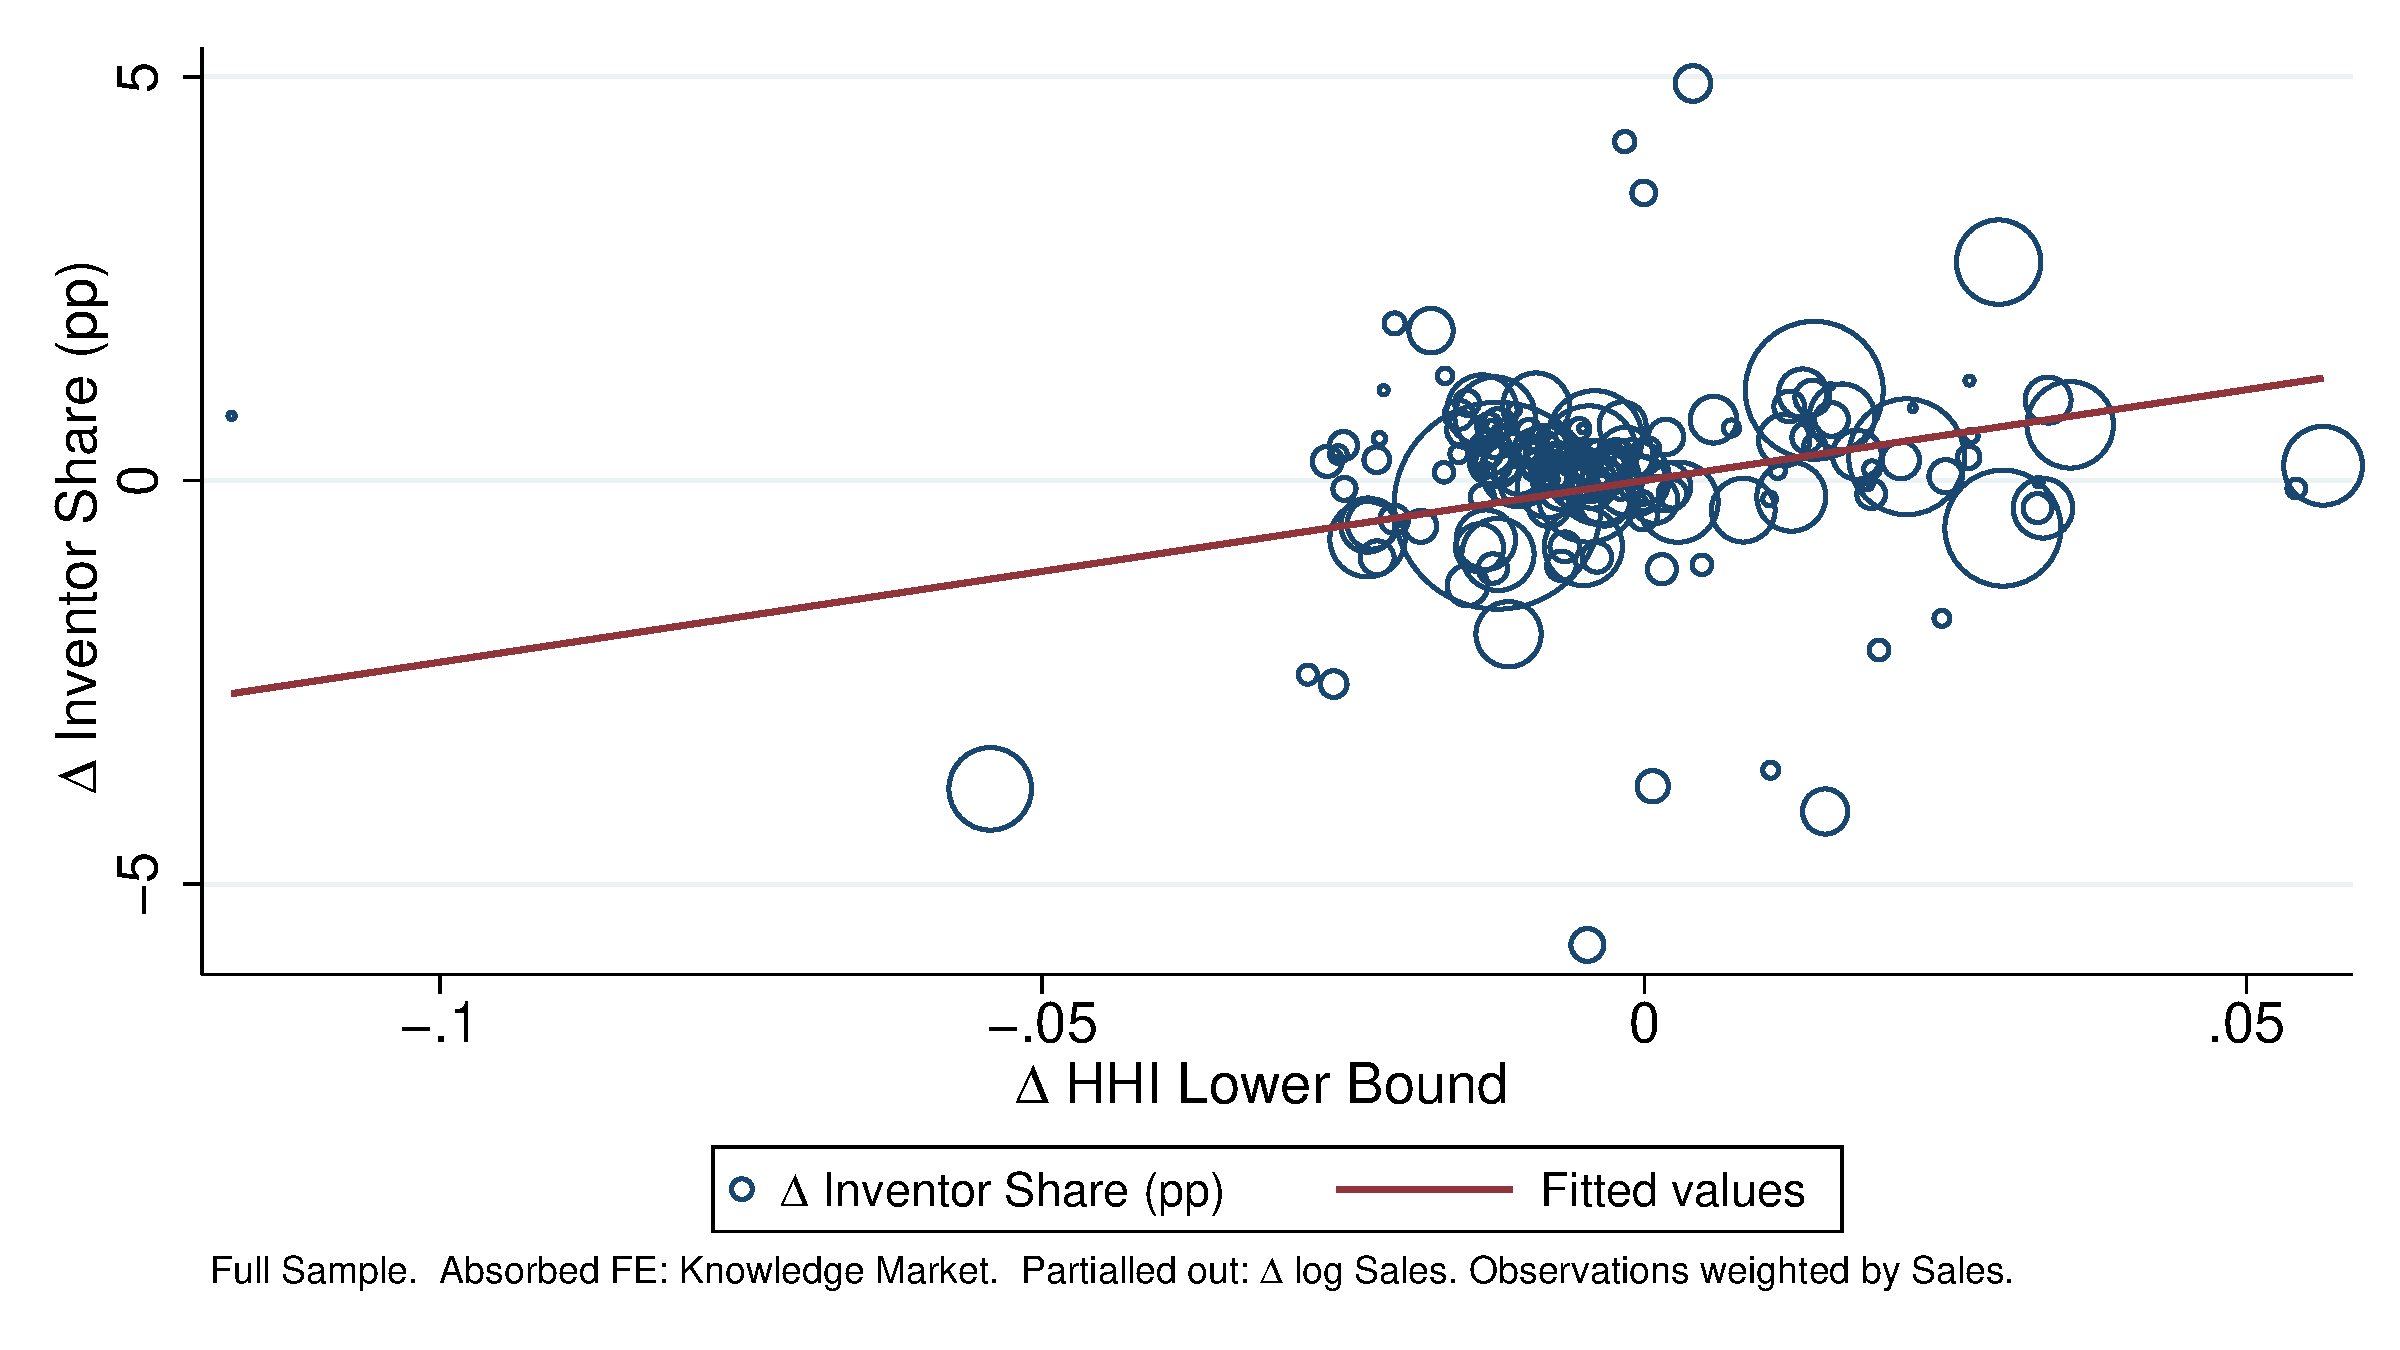
\includegraphics[width=0.9\textwidth]{../graphs/raw_Dk4_hhi_inv_fe10}}

\subfloat[Binned Scatter Plot, Specification in Column (6)]{\centering{}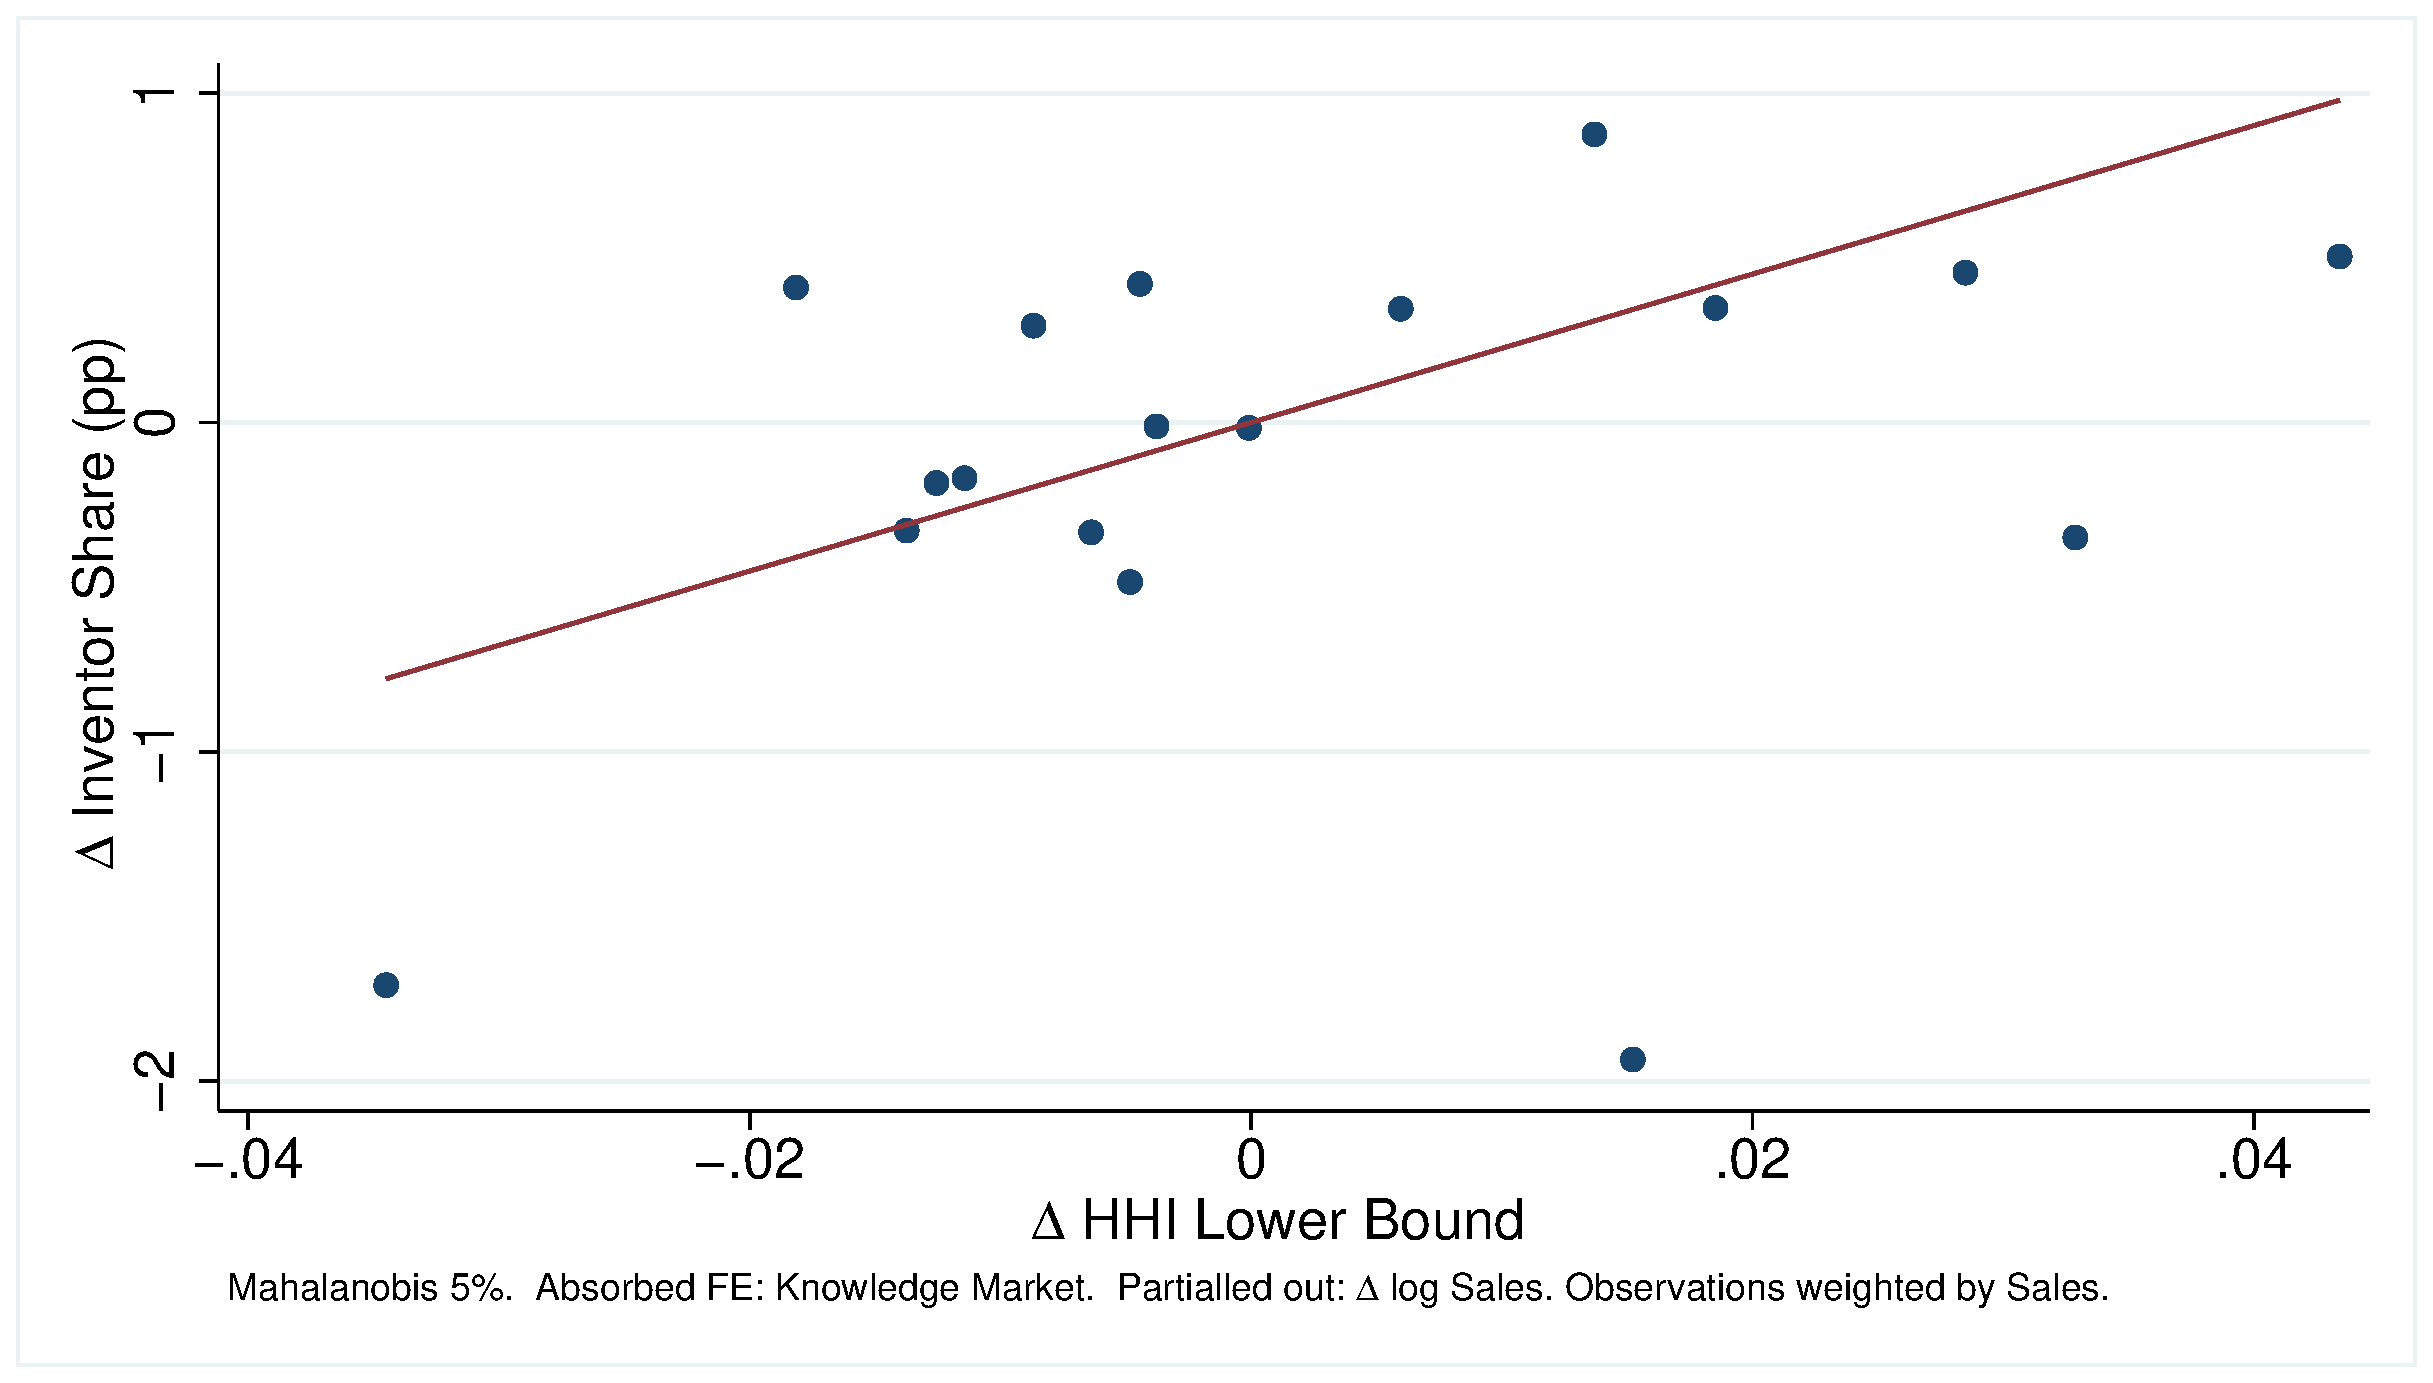
\includegraphics[width=0.9\textwidth]{../graphs/bin_Dk4_hhi_inv_fe12}}\\

\raggedright{}{\small{}Note: This figure presents residualized scatter
plots of the change in the share of effective inventors of sector
$p$ over total inventors in knowledge market $k$, over the change
in the lower bound of the Herfindal-Hirschman Index for product market
$p$, as implied by Census concentration ratios. The upper panel reports
the data for the full sample, where both variables are residualized
by change in log real sales and knowledge market fixed effects. The
size of the markers is proportional to the weight of each observation
in the regression (sector sales in 2012). The regression line uses
the coefficient on the change in HHI lower bound in Column (2) of
Table }\ref{tab: RegShInvHHI}{\small{}. The lower panel presents
a binned scatter plot removing the observations with the highest 5\%
Mahalanobis distance from the sample centroid. Observations are aggregated
using sales weights and the regression line is from Column (6) of
Table }\ref{tab: RegShInvHHI}{\small{}.}{\small\par}
\end{figure}


\paragraph{IV Results}

I now present instrumental variable results that suggest that the
relation between concentration and inventor shares is causal. Indeed,
more concentration could be the result of increasing technological
entry barriers as incumbents hire more R\&D inventors. In this scenario,
the causality would flow from increased inventor shares to higher
concentration. Above, I tried to mitigate this concern using as my
outcome variable the average share of inventors following the Economic
Census years to which the HHI refers. However, reverse causality could
still be present if the autocorrelation of inventor shares is sufficiently
high. As a consequence, I have calculated 2SLS estimates that instrument
the change in the HHI lower bound with changes in product market restrictions,
as measured by the Mercatus dataset RegData 4.0. Theoretically, an
increase in restrictions should raise barriers to entry in affected
product markets, thus leading to higher concentration. As discussed
below, such proves to be the case empirically, validating sector-specific
restrictions as an instrument for concentration. A violation of the
exclusion restriction requires a causal connection between product
market regulations and the share of inventors hired by each sector,
independent of product market concentration. For example, regulations
affecting existing technologies might require more inventors to meet
product market restrictions. However, this effect is unlikely to be
sufficiently large and persistent to be captured by my measure of
inventor shares. Further, the regulations counted in RegData are not
exclusively product restrictions, but also include reporting obligations
and other legal burdens that are not related to technological components.
In addition, while product restrictions might certainly induce a change
in the direction of innovation, there is no a priori reason to believe
that the scale of innovation activity should increase. These considerations
lead me to believe that the exclusion restriction is not likely to
be violated.

The results of the 2SLS estimation are presented in the upper panel
of Table \ref{tab: RegIV}. The specification is the same as in Column
(2) of \ref{tab: RegShInvHHI}, including both knowledge market and
sale change fixed effects. The 2SLS estimates confirm the significance
of concentration changes for the increase in knowledge market inventor
shares. The magnitudes of estimated coefficients are statistically
indistinguishable from the ones reported in the baseline regression.
The first-stage F clearly indicates that instruments are weak. This
is unsurprising since, as detailed above, both the HHI lower bound
and the regulation measures are estimated. In particular, I had to
impute regulations for a large part of the sample using the cosine-similarity
between product market restrictions.\footnote{Using only available sectors requires dropping two thirds of the observations.
See Appendix \ref{app: Data-Construction-Details} for details on
data construction.} However, instruments are not irrelevant. The results in the lower
panel of Table \ref{tab: RegIV} imply that the first-stage t-statistic
for the regression of the change in the HHI lower bound over log-regulations
is 2.07, which corresponds to a p-value of 0.041. The reduced form
regression of inventor share over log restriction change is as highly
significant. Accordingly, the SW underidentification test rejects
the null hypothesis at a 5\% confidence level. Given the weakness
of the instruments, I also report the Anderson-Rubin p-value and the
corresponding confidence intervals in brackets, which confirm that
the coefficient is 5\% significant.

Taken together, the results presented in this section establish a
causal link between the increase in inventor concentration and the
shifts in product market concentration across NAICS 4-digit sectors.

\begin{table}
\caption{IV Regressions of Change in 4-digit Knowledge Market Share over Change
in HHI Lower Bound, 2SLS Long-Difference, 1997-2012\label{tab: RegIV}}

\begin{centering}
\subfloat[2SLS Results]{
\centering{}\scalebox{.9}{{
\def\sym#1{\ifmmode^{#1}\else\(^{#1}\)\fi}
\begin{tabular}{l*{2}{c}}
\hline\hline
                    &$\Delta$ Inventor Share (pp)   &               \\
                    &\multicolumn{1}{c}{(1)}   &\multicolumn{1}{c}{(2)}   \\
\hline
$\Delta \underline{\text{HHI}}$&      32.426+  &      30.096+  \\
                    &    (16.987)   &    (15.819)   \\
                    &$\left[4.850,\  99.013\right]$   &$\left[4.415,\  92.104\right]$   \\
$\Delta \log$ Sales &               &       0.525*  \\
                    &               &     (0.247)   \\
                    &               &$\left[0.525,\  0.525\right]$   \\
\hline
Knowledge Market FE &   \ding{51}   &   \ding{51}   \\
Sample              & Full Sample   &Mahalanobis 5\%   \\
Weight              &       Sales   &       Sales   \\
Observations        &         157   &         150   \\
First-Stage F       &    4.656786   &    4.753009   \\
Anderson-Rubin p-value&    .0298009   &    .0321185   \\
\hline\hline
\end{tabular}
}
}}\\
\subfloat[First Stage and Reduced Form]{
\centering{}\scalebox{1}{{
\def\sym#1{\ifmmode^{#1}\else\(^{#1}\)\fi}
\begin{tabular}{l*{2}{c}}
\hline\hline
                    &Ch. 4d K.M. Eff. Inv. Share (\%)   &Ch. HHI lower bound   \\
                    &\multicolumn{1}{c}{(1)}   &\multicolumn{1}{c}{(2)}   \\
\hline
Ch. Log Restricitions (NAICS 4d)&       0.478*  &       0.016*  \\
                    &     (0.220)   &     (0.007)   \\
Ch. Log Real Sales  &       0.539+  &      -0.000   \\
                    &     (0.274)   &     (0.005)   \\
\hline
4D Knowledge Market FE&   \ding{51}   &   \ding{51}   \\
Sample              & Full Sample   & Full Sample   \\
Weight              &       Sales   &       Sales   \\
Observations        &         153   &         153   \\
\hline\hline
\end{tabular}
}
}}\\
\par\end{centering}
\raggedright{}{\small{}Note: Regressions weighted by sales in 2012;
robust standard errors in parentheses; symbols denote significance
levels $\left(+\ p<0.1,^{*}\ p<0.05,^{**}\ p<.01,^{***}\ p<.001\right)$;
checkmarks indicate the inclusion of fixed effects. This table presents
the results of specifications (\ref{eq: spec}), when the outcome
is the share of effective inventors of sector $p$ over total inventors
in knowledge market $k$, and the independent variable is the change
in the lower bound of the Herfindal-Hirschman Index for product market
$p$, as implied by Economic Census concentration ratios, instrumented
by the change in log-restrictions relevant to the NAICS sector. The
lower panel present first-stage and reduced-form relations. ``Full
Sample'' and ``Mahalanobis 5\%'' refer to the samples described
in the main text.}{\small\par}
\end{table}


\subsubsection{Sectors that Attracted More Researchers Saw Increasing Top Firms'
Inventor Shares and Falling Patent Forward Citations}

While the findings presented so far establish a connection between
inventor and product market concentration, they do not establish that
changes in the distribution of researchers across sectors are inefficient.
It would not be unreasonable, for example, to think that more concentrated
sectors saw increased entry as a result of the higher rents captured
by incumbents. Table \ref{tab: RegStats} shows that the opposite
occurred. Specifically, the share of effective inventors accruing
to top inventor-hiring firms increased in the sectors that attracted
more inventors over the period considered, relative to firms with
fewer inventors in the sector\textemdash a finding consistent across
a variety of measures displayed in Columns (1) to (6). These outcomes
suggest that inventors have increasingly concentrated among large
incumbents, that is, sectors that increased their inventor share also
saw a \emph{within-sector} increase in inventor concentration.

Throughout this section, I present results using changes in inventor
shares to focus directly on the correlation between inventor transitions
and their within-sector distribution. Unless otherwise noted, these
findings are robust to using the change in the HHI rather than the
inventor share, as should be expected from the strong correlation
between these two variables reported in previous tables. For this
section, and other patent-based measures, I present robustness results
using the change in the HHI in Appendix \ref{subsec:Patents-with-HHI}.

My next finding suggests that inventor concentration is driven by
a rise in defensive innovation, that is R\&D aimed at protecting the
incumbents' dominant position and raising barriers to entry. Table
\ref{tab: RegFwdCite} shows that inventors' concentration in specific
sectors went hand in hand with a fall in forward citations for patents,
a standard measure of a patent's contribution to further innovations
\citep{hallNBERPatentCitation2001}. The result in Columns (1) and
(2) report two different measures of forward citations that differ
in how the series are corrected for truncation. As discussed in Section
\ref{subsec:Other data and aggregation}, the measure in Column (2)
uses the procedure delineated by \citet{hallNBERPatentCitation2001},
computing the forward citation lag distribution conditioning on the
technology class of the cited patent. Column (2) also conditions on
the technology class of citing patents. Column (3) presents the estimates
relative to patent generality, a measure of patent impact that increases
with the scope of application. The regressions in this table are unweighted
since they rely only on patent data, but results are robust to using
the HHI as a regressor and weighting by sales. I present results for
the full sample, as well as restricting to the middle range of changes
in inventor shares, which contains more than 90\% of the observations.
In both samples, I find a highly significant negative relation between
changes in inventor shares and the fall in forward citations. The
coefficients imply a high semi-elasticity of self citations to changes
in the inventor shares, whereby a 1 percentage point increase in the
share of inventors leads to a 0.2-0.5\% reduction in forward citations.
After dropping extreme observations, I also find a significant decrease
in the generality of the patents, indicating that concentrating sectors
produce less widely applicable patents. However, the generality finding
is not robust to estimating the regression using the HHI as the independent
variable.

The fall in forward citations is a first indication of the presence
of defensive innovation \citep[see, e.g.,][]{guellecPreemptivePatentingSecuring2012}.
In the next section, I show that these patents also appear to do relatively
little to boost productivity, as measured by growth in output per
worker.

Before moving to the results on productivity, I investigate a competing
explanation for my findings on output growth. As highlighted by \citet{acemogluRadicalIncrementalInnovationForthcoming}
and \citet{akcigitGrowthHeterogeneousInnovations2018} among others,
large incumbents have a strong incentive to focus on improving their
own products at the expense of broadly applicable innovation. This
mechanism would also imply that an increase in incumbents' share of
R\&D resources leads to falling innovation productivity. In order
to assess the importance of this channel, and in keeping with the
analysis in \citet{akcigitGrowthHeterogeneousInnovations2018}, I
use the share of self-citations to measure the extent of internal
innovation conducted by firms. Table \ref{tab: RegSelfCite} displays
the results pertaining to this measure. All columns use as dependent
variable the change in excess log self-citations as defined in Section
\ref{subsec:Other data and aggregation}. Columns (1) and (2) build
excess self-citations correcting for the importance of firms' patents
for the CPC group, which reflects the technological classification
of the patent. Columns (3) and (4) use the more narrowly defined CPC
subgroups for robustness. Coefficients are mostly non-significant
and turn negative when knowledge market fixed effects are included.
Column (3) displays a marginally significant coefficient. However,
this result is not robust to using the HHI as regressor and weighting
regressions by sales as in the baseline specification. The findings
in this table suggest that incremental innovation does not drive my
results.

\begin{sidewaystable}[ph]
\caption{Regressions of Change in Inventor Distribution Measures over Change
in 4-digit Knowledge Market Share, Long-Difference, 1997-2012\label{tab: RegStats}}

\begin{centering}
\scalebox{1}{{
\def\sym#1{\ifmmode^{#1}\else\(^{#1}\)\fi}
\begin{tabular}{l*{2}{c}*{3}{H}}
\hline\hline
                    &Ch. Inv. 90/50 Quantile Ratio   &$\Delta$ Top 10\%/Bottom 50\%   &Ch. Inv. Top-50/Bottom-50 Share Ratio   &$\Delta$ Top 10\%   &$\Delta$ Bottom 50\%   \\
                    &\multicolumn{1}{c}{(1)}   &\multicolumn{1}{c}{(2)}   &\multicolumn{1}{H}{(3)}   &\multicolumn{1}{H}{(4)}   &\multicolumn{1}{H}{(5)}   \\
\hline
$\Delta$ Inventor Share (pp)&       0.211+  &       0.243*  &       0.314+  &       0.018** &      -0.008*  \\
                    &     (0.107)   &     (0.097)   &     (0.184)   &     (0.006)   &     (0.004)   \\
$\Delta \log$ Sales &      -0.100   &       0.328   &       0.147   &       0.026   &       0.005   \\
                    &     (0.122)   &     (0.294)   &     (0.316)   &     (0.020)   &     (0.007)   \\
\hline
Knowledge Market FE &   \ding{51}   &   \ding{51}   &   \ding{51}   &   \ding{51}   &   \ding{51}   \\
Sample              & Full Sample   & Full Sample   & Full Sample   & Full Sample   & Full Sample   \\
Weight              &       Sales   &       Sales   &       Sales   &       Sales   &       Sales   \\
Observations        &         118   &         118   &         118   &         118   &         118   \\
\hline\hline
\end{tabular}
}
}\\
\par\end{centering}
\raggedright{}{\small{}Note: Regressions weighted by sales in 2012;
robust standard errors in parentheses; symbols denote significance
levels $\left(+\ p<0.1,^{*}\ p<0.05,^{**}\ p<.01,^{***}\ p<.001\right)$;
checkmarks indicate the inclusion of fixed effects. Please refer to
notes in Table \ref{tab: RegShInvHHI} for further details. Column
(1) uses the ratio in the 90 percentile of effective inventors to
the median as the outcome variable. Columns (2) and (3) instead present
the share ratio, that is the share of effective inventors accruing
to the top 10 or 50\% relative to the share accruing to the bottom
50\% of the distribution within each NAICS sector.}{\small\par}
\end{sidewaystable}

\begin{table}
\caption{Regressions of Changes in Forward Citation over 4-digit Knowledge
Market Share, Long-Differences, 1997-2012\label{tab: RegFwdCite}}

\begin{centering}
\subfloat[Full sample]{\begin{centering}
\par\end{centering}
\centering{}\scalebox{.9}{{
\def\sym#1{\ifmmode^{#1}\else\(^{#1}\)\fi}
\begin{tabular}{l*{3}{c}}
\hline\hline
                    &Ch. in log citations per patent (CPC2 based)   &Ch. in log citations per patent (Total)   &Ch. in patent generality   \\
                    &\multicolumn{1}{c}{(1)}   &\multicolumn{1}{c}{(2)}   &\multicolumn{1}{c}{(3)}   \\
\hline
Ch. 4d K.M. Eff. Inv. Share (\%)&      -0.197***&      -0.227***&      -0.004   \\
                    &     (0.044)   &     (0.051)   &     (0.004)   \\
Ch. Log Real Sales  &      -0.234*  &      -0.258+  &       0.008   \\
                    &     (0.112)   &     (0.148)   &     (0.013)   \\
\hline
4D Knowledge Market FE&   \ding{51}   &   \ding{51}   &   \ding{51}   \\
Sample              & Full Sample   & Full Sample   & Full Sample   \\
Weight              &               &               &               \\
Observations        &         153   &         153   &         153   \\
\hline\hline
\end{tabular}
}
}}
\par\end{centering}

\begin{centering}
\subfloat[Full sample, restricting to the middle range of the change in inventor
shares ($-2\%$ to $+2\%$)]{\centering{}\scalebox{.9}{ {
\def\sym#1{\ifmmode^{#1}\else\(^{#1}\)\fi}
\begin{tabular}{l*{3}{c}}
\hline\hline
                    &$\Delta \log$ Citations/Patent (CPC)   &$\Delta \log$ Citations/Patent (Total)   &$\Delta$ Patent Generality   \\
                    &\multicolumn{1}{c}{(1)}   &\multicolumn{1}{c}{(2)}   &\multicolumn{1}{c}{(3)}   \\
\hline
$\Delta$ Inventor Share (pp)&      -0.545***&      -0.618***&      -0.025*  \\
                    &     (0.113)   &     (0.137)   &     (0.012)   \\
$\Delta \log$ Sales &      -0.232*  &      -0.255+  &       0.008   \\
                    &     (0.109)   &     (0.146)   &     (0.012)   \\
\hline
Knowledge Market FE &   \ding{51}   &   \ding{51}   &   \ding{51}   \\
Sample              & Full Sample   & Full Sample   & Full Sample   \\
Weight              &               &               &               \\
Observations        &         144   &         144   &         144   \\
\hline\hline
\end{tabular}
}
}}\\
\par\end{centering}
\raggedright{}{\small{}Note: Unweighted regressions; robust standard
errors in parentheses; symbols denote significance levels $\left(+\ p<0.1,^{*}\ p<0.05,^{**}\ p<.01,^{***}\ p<.001\right)$;
checkmarks indicate the inclusion of fixed effects. This table present
the results of specification (\ref{eq: spec}), when the outcome is
the log-change in forward citations and the change in patent generality
in sector $p$ over the change in the share of inventors employed
in sector $p$. Column (1) and (2) presents the results when forward
citations are extrapolated the procedure Hall et al. (2000) to avoid
truncation bias. A specific cite-lag distribution over 35 years is
estimated for each pair of cited and citing CPC2-codes. Column (1)
employs the extrapolation scheme by each pair of CPC2 cited and citing
sector. Column (2) applies the extrapolation scheme to total citations
received by each cited patent. Column (3) presents results on the
patent generality measures. All columns exclude self-citations. Upper
panel: full sample; bottom panel: excluding sectors with absolute
increase in the inventor share above 2\%.}{\small\par}
\end{table}
\begin{table}
\caption{Regressions of Change in Excess Self-Citations over 4-digit Knowledge
Market Share, Long-Differences, 1997-2012\label{tab: RegSelfCite}}

\begin{centering}
\scalebox{.9}{{
\def\sym#1{\ifmmode^{#1}\else\(^{#1}\)\fi}
\begin{tabular}{l*{4}{c}}
\hline\hline
                    &$\Delta$ CPC group self-citations   &               &$\Delta$ CPC subgroup self-citations   &               \\
                    &\multicolumn{1}{c}{(1)}   &\multicolumn{1}{c}{(2)}   &\multicolumn{1}{c}{(3)}   &\multicolumn{1}{c}{(4)}   \\
\hline
$\Delta$ Inventor Share (pp)&       0.920   &      -0.444   &       0.958+  &      -0.228   \\
                    &     (0.711)   &     (1.083)   &     (0.512)   &     (0.801)   \\
$\Delta \log$ Sales &      -1.841   &      -1.954   &      -1.456   &      -1.674   \\
                    &     (1.925)   &     (1.988)   &     (1.326)   &     (1.279)   \\
\hline
Knowledge Market FE &               &   \ding{51}   &               &   \ding{51}   \\
Sample              & Full Sample   & Full Sample   & Full Sample   & Full Sample   \\
Weight              &               &               &               &               \\
Observations        &         157   &         153   &         157   &         153   \\
\hline\hline
\end{tabular}
}
}
\par\end{centering}
\begin{centering}
\par\end{centering}
\raggedright{}{\small{}Note: Unweighted regressions; robust standard
errors in parentheses; symbols denote significance levels $\left(+\ p<0.1,^{*}\ p<0.05,^{**}\ p<.01,^{***}\ p<.001\right)$;
checkmarks indicate the inclusion of fixed effects. This table presents
the results of specifications (\ref{eq: spec}), when the outcome
is the change in excess self-citations in sector $p$ over the change
in the share of inventors employed in sector $p$. }{\small\par}
\end{table}
\FloatBarrier

\subsubsection{Markets with Growing Inventor Shares Experienced a Fall in Inventor
Productivity}

Table \ref{tab: RegProd} presents the results of running (\ref{eq: spec})
when the outcome is the average growth in output per worker per effective
inventor. I use growth in annual output per worker provided by the
Economic Census and average this measure over the five-year window
starting in the Economic Census year, and I analogously build a measure
of average effective inventors over the same period. Inventor productivity
is then defined as average output per worker growth divided by average
number of effective inventors. Both the outcome and the dependent
variable are measured in percentage points. Table \ref{tab: RegProd}
reveals a negative and significant correlation between the increase
in the number of effective inventors and inventor productivity, regardless
of the independent variable employed and the sample restriction adopted.

Starting from the upper panel of Table \ref{tab: RegProd}, the median
change in the share of effective inventors over the period was $.014\text{pp}$,
while the measure of effective inventors has a median of 2018.\footnote{Recall that effective inventors in each year are measured as the sum
of inventor fixed-effects in each year, and therefore do not represent
the simple count of inventors.} The coefficient for concentration in Column (4) implies a fall of
$.15\text{pp}$ ($-.005\times.014\text{pp}\times2018$) in average
annual labor productivity growth. This number decreases to $-.28\text{pp}$
when considering only sectors with positive growth in labor productivity,
which accounted for the bulk of the increase in inventor shares. An
alternative back-of-the-envelope computation, using the change in
product market concentration to predict the change in inventor shares
gives even starker results. Using the coefficient in Column (2) of
Table \ref{tab: RegShInvHHI}(a) and considering a median change in
the HHI of $0.002$ yields an increase in the share of effective inventors
in concentrating sectors of $0.045\text{pp}$. This implies a fall
in average labor productivity implied by misallocation of 0.45pp.
While these numbers might appear large considering the entirety of
the economy, it is worth noting that my sample includes mainly manufacturing
and retail sectors, which experienced a sizable reduction of $2.73pp$
in average annual productivity growth from 1997 to 2012, driven by
a steep decline in output per worker growth in manufacturing. Therefore,
the mechanism I propose would explain around 15 percent of the observed
decrease in output per worker growth in these sectors.

The estimates in the lower panel of Table \ref{tab: RegProd}, which
uses the HHI instead the change in inventor shares as independent
variable, imply even larger growth effects. Using the estimates in
Column (2), a median HHI change of 0.02 and a median number of effective
inventors of 1421 in sectors with growth in inventor shares implies
a $-0.78$pp change in output per worker growth from misallocation,
with a confidence interval ranging from $-0.13$pp to $-1.45$pp.
The midpoint of these estimates would explain $28.6\%$ of the observed
fall in output per worker growth over the sample period ($-2.73\text{pp}$),
with bounds ranging from $4.8\%$ to $53\%$.

This last set of results further supports the hypothesis that defensive
innovation increased in concentrating sectors. To protect their dominant
position, firms engage in such R\&D to thwart innovation by potential
competitors. Similarly citing defensive innovation as a motive, \citet{argentePatentsProductsProduct2020a}
report that incumbent firms tend to register a large number of patents,
but account for a small share of overall innovations.

\begin{table}[h]
\caption{Regressions of Changes in Inventor Productivity over Changes in Inventors'
Share and HHI, Long-Difference, 1997-2012\label{tab: RegProd}}

\begin{centering}
\subfloat[Change in Inventors' Share as Independent Variable]{
\centering{}\scalebox{.95}{{
\def\sym#1{\ifmmode^{#1}\else\(^{#1}\)\fi}
\begin{tabular}{l*{4}{c}}
\hline\hline
                    &$\Delta$ Growth/Inventor (pp)   &               &               &               \\
                    &\multicolumn{1}{c}{(1)}   &\multicolumn{1}{c}{(2)}   &\multicolumn{1}{c}{(3)}   &\multicolumn{1}{c}{(4)}   \\
\hline
$\Delta \underline{HHI}$  &      -0.332** &      -0.292*  &      -0.332** &      -0.290*  \\
                    &     (0.113)   &     (0.123)   &     (0.114)   &     (0.126)   \\
$\Delta \log$ Sales  &               &      -0.052*  &               &      -0.053*  \\
                    &               &     (0.021)   &               &     (0.022)   \\
\hline
Knowledge Market FE&   \ding{51}   &   \ding{51}   &   \ding{51}   &   \ding{51}   \\
Sample              & Full Sample   & Full Sample   &Mahalanobis 5\%   &Mahalanobis 5\%   \\
Weight              &       Sales   &       Sales   &       Sales   &       Sales   \\
Observations        &         101   &         101   &          98   &          94   \\
\hline\hline
\end{tabular}
}
}}\\
\subfloat[Change in HHI as Independent Variable]{
\centering{}\scalebox{.95}{{
\def\sym#1{\ifmmode^{#1}\else\(^{#1}\)\fi}
\begin{tabular}{l*{4}{c}}
\hline\hline
                    &$\Delta$ Growth/Inventor (pp)   &               &               &               \\
                    &\multicolumn{1}{c}{(1)}   &\multicolumn{1}{c}{(2)}   &\multicolumn{1}{c}{(3)}   &\multicolumn{1}{c}{(4)}   \\
\hline
$\Delta \underline{\text{HHI}}$&      -0.332** &      -0.292*  &      -0.332** &      -0.290*  \\
                    &     (0.113)   &     (0.123)   &     (0.114)   &     (0.126)   \\
$\Delta \log$ Sales &               &      -0.052*  &               &      -0.053*  \\
                    &               &     (0.021)   &               &     (0.022)   \\
\hline
Knowledge Market FE &   \ding{51}   &   \ding{51}   &   \ding{51}   &   \ding{51}   \\
Sample              & Full Sample   & Full Sample   &Mahalanobis 5\%   &Mahalanobis 5\%   \\
Weight              &       Sales   &       Sales   &       Sales   &       Sales   \\
Observations        &         101   &         101   &          98   &          94   \\
\hline\hline
\end{tabular}
}
}}\\
\par\end{centering}
\raggedright{}{\small{}Note: Regressions weighted by sales in 2012;
robust standard errors in parentheses; symbols denote significance
levels $\left(+\ p<0.1,^{*}\ p<0.05,^{**}\ p<.01,^{***}\ p<.001\right)$;
checkmarks indicate the inclusion of fixed effects. Please refer to
notes in Table \ref{tab: RegShInvHHI} for further details. Inventor
productivity is measured as the average growth in output per worker
over the five years starting in the Economic Census year over the
total number of effective inventors in each sector. The upper panel
presents estimates when the independent variable is the change in
the share of inventors accruing to a sector, while the bottom panel
uses the change in the lower bound of the HHI index.}{\small\par}
\end{table}
\FloatBarrier
\end{document}
